\documentclass{article}

\usepackage{a4wide}
\usepackage[T1]{fontenc}
\usepackage[spanish]{babel}
\usepackage[utf8]{inputenc}
\usepackage{listings}
\usepackage{color}
\usepackage[math]{iwona}

\usepackage{graphics}
\usepackage{graphicx}

\usepackage{hyperref}

\newcommand{\code}[1]{\lstinline{#1}}

\definecolor{mygreen}{rgb}{0,0.6,0}
\definecolor{mygray}{rgb}{0.75,0.75,0.75}
\definecolor{mymauve}{rgb}{0.58,0,0.82}

\lstset{ %
  basicstyle=\ttfamily,
  backgroundcolor=\color{mygray},
  language=Python,
  showspaces=false, 
  showstringspaces=false,
  showtabs=false,
  numbers=left,                   
  numbersep=5pt,                  
  numberstyle=\tiny\color{mygreen},
  rulecolor=\color{black},              
  stepnumber=1,
  keywordstyle=\color{blue}  
}

\title{Manual de estilo}


\begin{document}
\maketitle

Los programas son ejecutados por máquinas, pero han de
ser leídos y mantenidos por humanos. Es necesario, por tanto, escribir
programas que sean fáciles de leer y en los que sea sencillo entender
la estructura y la lógica del mismo, es decir, saber qué hace y cómo lo hace.

A continuación damos una serie de pautas y convenciones que ayudan a la legibilidad y comprensión de los programas. Intentaremos seguir estas normas en todos los programas que aparezcan a lo largo de la asignatura.

\section{Nombres y comentarios}
\begin{itemize}
\item Por claridad, para aumentar la legibilidad y evitar problemas con caracteres especiales (como acentos), los nombres de funciones y variables estarán escritos en inglés.
\item Los nombres de variables serán aclaratorios. Ejemplos de nombres claros son: \code{maximum}, \code{radius}, \code{area}, \code{speed}. Ejemplos de nombres confusos son: \code{a1}, \code{c}, \code{xxx}. Las variables índice usadas para recorrer bucles pueden tener nombres sencillos y similares a los que clásicamentes se utilizan en matemáticas: \code{i}, \code{j}, \code{k}.
\item En muchas ocasiones, al definir con precisión un identificador para funciones o variables utilizamos varias palabras. En  estos casos, las palabras que componen el identificador se unirán con un guión bajo. Por ejemplo: \code{min_distance}, \code{shortest_path}, \code{validate_data}\ldots
\item Todo el texto que aparezca en el programa para explicar el mismo (comentarios, docstring, etc.), también estará escrito en inglés.
\end{itemize}

\section{Funciones}
\begin{itemize}
\item Todas las funciones deben estar documentadas en inglés explicando qué hacen, qué argumentos aceptan y qué devuelven. Este comentario, que se conoce como \emph {docstring} debe cumplir el formato que muestra la figura~\ref{fig:docstring}. Este formato de comentarios está basado en
\href{https://github.com/numpy/numpy/blob/master/doc/HOWTO_DOCUMENT.rst.txt}{numpydoc}


\begin{figure}
  \centering
 \begin{lstlisting}
def average(a, b):
    """
    Given two numbers a and b, return their average value.

    Parameters
    ----------
    a : number (int or float)
      Firsts number
    b : number (int or float)
      Second number

    Returns
    -------
    float
      The average value of a and b

    Example
    -------
    >>> average(5, 10)
    7.5
    """
    return (a + b) / 2.0
\end{lstlisting}
  \caption{Ejemplo de docstring para una función}
  \label{fig:docstring}
\end{figure}


Esta forma de comentar es muy importante, pues las diferentes herramientas que utilicemos para programar en python generan documentación a partir de la información contenida en el docstring. En Spyder, por ejemplo, la documentación de la función anterior se vería como aparece en la figura~\ref{fig:docstring_spyder}.

\begin{figure}
  \centering
  %\includegraphics[width=\textwidth]{docstring.jpeg} 
  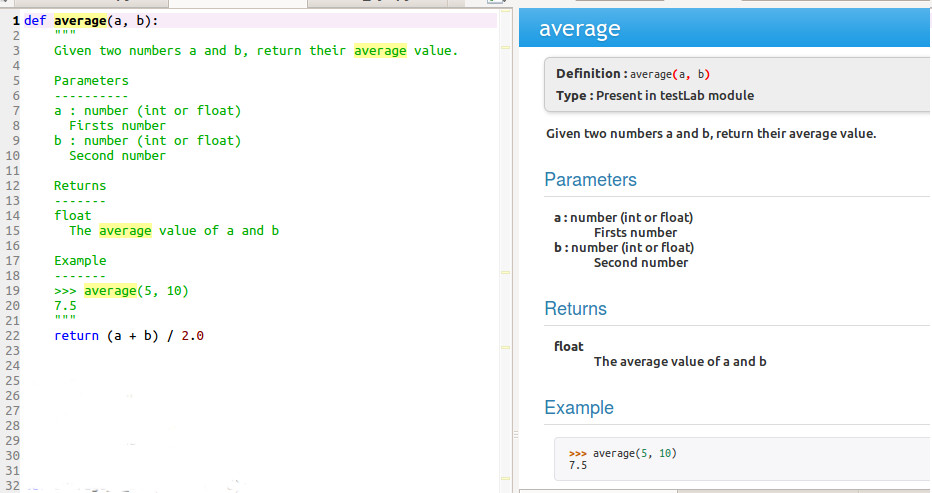
\includegraphics[scale=0.45]{ejcomment.jpg}
  \caption{Ejemplo de visualización del docstring de una función en Spyder}
  \label{fig:docstring_spyder}
\end{figure}

%\item Salvo en funciones recursivas, las funciones tendrán una única instrucción \code{return} al final de su cuerpo. No se permite devolver valores en otros puntos de la función.

\item  Dentro del cuerpo de las funciones se usarán los parámetros de la función o variables localmente definidas, no se usarán variables globales.
\end{itemize}


\section{Espaciado y separación}
\begin{itemize}
\item Solo habrá una instrucción por línea
\item Se importarán los módulos en líneas separadas. Por ejemplo:
\begin{lstlisting}
import string
from PIL import Image
\end{lstlisting}
\item Las lineas de texto no pueden ocupar más de 80 caracteres

\item Habrá 2 líneas en blanco para separar funciones

\item Como norma general, se dejará un espacio entre el operador y los operandos, incluido el operador de asignación. Ejemplos (el símbolo \texttt{\char32} representa un espacio):
\begin{lstlisting}[showspaces=true]
pi = 3.14
area = side * side
\end{lstlisting}
Ejemplos de expresiones que no cumplen este estilo son:
\begin{lstlisting}[showspaces=true]
pi=3.14
pi =3.14
area = side*side
\end{lstlisting}
En expresiones más complejas, es posible que juntar operadores y operandos, de forma uniforme y cuidadosa, mejore la legibilidad. Por ejemplo, la expresión 
 \begin{lstlisting}[showspaces=true]
y = (a*f - c*e)/(-c*b + a*d)
\end{lstlisting}
puede ser más fácil de leer y entender que 
\begin{lstlisting}[showspaces=true]
y = (a * f - c * e) / (-c * b + a * d)
\end{lstlisting}

\item Al invocar o definir funciones no se dejará ningún espacio al lado de los paréntesis. Los argumentos se separarán con una coma seguida de un espacio. Ejemplos:
\begin{lstlisting}[showspaces=true]
def maximun(a, b):
maximum(3, 45)
\end{lstlisting}
Ejemplos que no cumplen este estilo son:
\begin{lstlisting}[showspaces=true]
def maximun(a,b):
def maximun( a,b ):
def maximun( a, b ):
maximum(3,45)
maximum( 3,45)
maximum( 3, 45 )
maximum( 3,45 )
\end{lstlisting}
\end{itemize}
\end{document}
